\documentclass[twoside]{report}
\usepackage[a4paper,left=1.2in,right=0.8in,top=1.2in,bottom=0.8in]{geometry}
\linespread{1.5}
\usepackage{graphicx}
\usepackage{hyperref}
\usepackage{inputenc}
\usepackage{acro}
\usepackage{titlesec}
\usepackage{setspace}
\usepackage{amsmath}
\usepackage{amssymb}
\usepackage{subcaption}
\usepackage{fancyhdr}
\usepackage{array}

\fancyhf{}
\fancyhead[LE,RO]{\nouppercase{\leftmark\hfill\rightmark}}
\fancyfoot[C]{\thepage}

\graphicspath{{ /images}}
\renewcommand*\thesection{\arabic{section}}
\setcounter{secnumdepth}{3}
\setcounter{tocdepth}{3}
\renewcommand{\bibname}{References}
\newcolumntype{M}[1]{>{\centering\arraybackslash}m{#1}}

\title{TAKALEM : Deep learning approach for Algerian sign language recognition}
\author{Fathi Abdelmalek}
\date{\today}


\DeclareAcronym{sl}{
	short={SL},
	long={Sign language}
}
\DeclareAcronym{asp}{
	short={ASP},
	long={Algerian sign language}
}
\DeclareAcronym{ajs}{
	short={AJSL},
	long={Algerian jewish sign language}
}
\DeclareAcronym{fsl}{
	short={FSL},
	long={French sign language}
}
\DeclareAcronym{asl}{
	short={ASL},
	long={American sign language}
}
\DeclareAcronym{bsl}{
	short={BSL},
	long={British sign language}
}
\DeclareAcronym{jsl}{
	short={JSL},
	long={Japanese sign language}
}
\DeclareAcronym{slr}{
	short={SLR},
	long={Sign language recognition}
}
\DeclareAcronym{slt}{
	short={SLT},
	long={Sign language translation}
}
\DeclareAcronym{ai}{
	short={AI},
	long={Artificial Intelligence},
}
\DeclareAcronym{ml}{
	short={ML},
	long={Machine Learning},
}
\DeclareAcronym{knn}{
	short={KNN},
	long={K-nearest neighbors}
}
\DeclareAcronym{dtw}{
	short={DTW},
	long={Dynamic time wrapping}
}
\DeclareAcronym{hsbn}{
	short={HSBN},
	long={Handshape Bayesian Network}
}
\DeclareAcronym{dl}{
	short={DL},
	long={Deep Learning},
}
\DeclareAcronym{nn}{
	short={NN},
	long={Neural Network}
}
\DeclareAcronym{ann}{
	short={ANN},
	long={Artificial Neural Network}
}
\DeclareAcronym{mlp}{
	short={MLP},
	long={multilayer perceptrons}
}
\DeclareAcronym{dnn}{
	short={DNN},
	long={Deep Neural Network},
}
\DeclareAcronym{cnn}{
	short={CNN},
	long={Convolutional Neural Network},
}
\DeclareAcronym{tcn}{
	short={TCN},
	long={Temporal Convolutional Network}
}
\DeclareAcronym{ctc}{
	short={CTC},
	long={Connectionist Temporal Classification}
}
\DeclareAcronym{rnn}{
	short={RNN},
	long={Recurrent Neural Network},
}
\DeclareAcronym{lstm}{
	short={LSTM},
	long={Long-Short Term Memory},
}
\DeclareAcronym{svm}{
	short={SVM},
	long={Support Vector Machines},
}
\DeclareAcronym{hmm}{
	short={HMM},
	long={Hidden Markov Model}
}
\DeclareAcronym{nlp}{
	short={NLP},
	long={Natural Language Processing}
}
\DeclareAcronym{crf}{
	short={CRF},
	long={Conditional Random Field},
}
\DeclareAcronym{vr}{
	short={VR},
	long={Virtual Reality},
}
\DeclareAcronym{ar}{
	short={AR},
	long={Augmented Reality},
}
\DeclareAcronym{imu}{
	short={IMU},
	long={Inertial Measurement Unit},
}
\DeclareAcronym{mems}{
	short={MEMS},
	long={Micro Electro-Mechanical Systems},
}
\DeclareAcronym{dmp}{
	short={DMP},
	long={Digital Motion Processor},
}
\DeclareAcronym{soc}{
	short={SoC},
	long={system-on-a-chip},
}
\DeclareAcronym{iot}{
	short={IoT},
	long={Internet of Things},
}

\begin{document}
	\pagestyle{plain}
	\makeatletter
	\begin{titlepage}
	\begin{center}
		PEOPLE’S DEMOCRATIC REPUBLIC OF ALGERIA\\[0.4cm]
		MINISTRY OF HIGHER EDUCATION AND SCIENTIFIC RESEARCH\\[0.4cm]
		LARBI TEBESSI UNIVERSITY\\[0.4cm]
		
\includegraphics[width=0.25\textwidth]{./images/univ-tebessa.jpg}\\[1cm]
		FACULTY OF EXACT SCIENCES AND SCIENCES OF NATURE AND LIFE\\[0.4cm]
		DEPARTMENT OF MATHEMATICS AND COMPUTER SCIENCE\\[0.5cm]
		\rule{\textwidth}{0.075cm}\\[0.4cm]
		\textsc{\huge \bfseries \@title}\\[1cm] 
		\rule{\textwidth}{0.075cm}\\[1cm]
		\begin{minipage}{0.4\textwidth}
			\begin{flushleft}
				\emph{\textbf{Submitted by}}\\
				\textsc{\@author}
			\end{flushleft}
		\end{minipage}
		\begin{minipage}{0.4\textwidth}
			\begin{flushright}
				\emph{\textbf{Supervised by}}\\
				\textsc{Pr. Mohamed Amroun}\\
				\textsc{Dr. Issam Bendib}
			\end{flushright}
		\end{minipage}
		\vfill
		\@date
	\end{center}
\end{titlepage}

	\makeatother
	\newpage
	\thispagestyle{empty}
	\mbox{}
	\newpage
	\pagenumbering{roman}
	\newenvironment{dedication}
{
	\thispagestyle{empty}
	\vspace*{\stretch{1}}
	\itshape
	\raggedleft
}
{\par
	\vspace{\stretch{3}}
	\clearpage
}
\begin{center}
	\section*{Dedication}
\end{center}
\begin{dedication}
	To my dear mother
	
	To my dear father
	
	To my sisters and brothers
	
	To my adorable grandmother
	
	To my friends and colleagues
	
	To every one who have supported me
	\par
	\vspace{2\baselineskip}
	
	\vspace{\baselineskip}
	\usefont{T1}{LobsterTwo-LF}{bx}{it}
	FATHI ABDELMALEK
\end{dedication}
	\clearpage
	\tableofcontents
	\clearpage
	\listoffigures
	\clearpage
	\listoftables
	\clearpage
	\printacronyms
	\clearpage
	\begin{abstract}
	
	Sign language recognition (SLR) has been a challenging task due to the complexity of hand gestures and the variability among sign languages. This thesis presents Takalem gloves, a wearable device designed for SLR using deep learning techniques. The proposed architecture consists of two ESP32 microcontrollers, flex sensors, IMUs, and a speaker. The dataset was collected using the gloves and preprocessed using Python. The deep learning model is based on convolutional and recurrent neural networks and was trained and evaluated on the American Sign Language dataset. The results showed an accuracy of 97.5\% on a test set of 1,200 signs. The proposed approach has the potential to enhance the communication between the hearing-impaired and the hearing communities, and can be further developed for other sign languages.
\end{abstract}
\providecommand{\keywords}[1]
{
	\small	
	\textbf{\textit{Keywords---}} #1
}
\keywords{sign language recognition, artificial intelligence, machine learning, deep learning}
	\clearpage
	\section*{Acknowledgements}
\paragraph{}
I would like to take this opportunity to express my sincere gratitude to all those who have supported and guided me throughout this incredible journey.

First and foremost, I extend my deepest appreciation to the members of the LAMIS laboratory at Echahid Cheikh Larbi Tebessi University of Tebessa. I am immensely grateful to my supervisor Professor Mohammed Amroune, Dr. Issam Bendib, Dr. M. Yassin Haouam, Dr. Khelifa Boudjemaa, and Dr. Salima Bourougaa for their invaluable guidance, encouragement, and support throughout this project. Their expertise and mentorship have been instrumental in shaping my research and academic development.

I would also like to extend my heartfelt thanks to all the professors, researchers, and fellow students at LAMIS laboratory for their collaboration, insightful discussions, and constructive feedback. Their collective efforts have greatly enriched my understanding and contributed to the success of this work.

Furthermore, I am deeply indebted to the faculty and staff of the university for providing a conducive academic environment and research facilities. Their commitment to excellence and dedication to fostering knowledge and innovation have played a significant role in the realization of this project.

I would like to express my gratitude to my family and friends for their unwavering support, patience, and belief in me. Their encouragement and understanding have been my source of strength throughout this challenging endeavor.

Finally, I would like to thank Hisham Kada Medjahed who gave us a training course in Arduino, thanks to which I was able to deal with sensors efficiently and effectively.

Although it is not possible to mention everyone individually, please know that your support and contributions have been deeply appreciated.

Thank you all for being a part of this remarkable journey and for your unwavering support.

Sincerely,
Fathi Abdelmalek

	\clearpage
	\pagenumbering{arabic}
	\pagestyle{fancy}
	\addcontentsline{toc}{chapter}{General Introduction}
	\chapter*{General Introduction}
\section{Context of Work}
\paragraph{}
\ac{slr} is a rapidly evolving field that aims to enable effective communication between individuals with hearing impairments who use \ac{sl} and those who do not. \ac{sl}, including \ac{asp}, are visual languages that rely on hand gestures, facial expressions, and body movements to convey meaning. Recognizing and interpreting \ac{sl} gestures accurately is essential for facilitating inclusive communication and ensuring equal access to information and services for the deaf community.
\paragraph{}
In recent years, advancements in \ac{dl} have revolutionized \ac{slr}. \ac{dl} models, particularly \ac{cnn} and \ac{rnn}, have shown remarkable success in analyzing and understanding complex visual data, making them well-suited for \ac{slr} tasks. By training \ac{dl} models on large \ac{sl} datasets, researchers have achieved significant improvements in accuracy and real-time recognition.
\paragraph{}
However, the development of accurate and robust \ac{slr} systems, especially for less-studied \ac{sl}s like \ac{asp}, remains a challenge. \ac{asp} has its unique vocabulary, grammar, and cultural aspects, which necessitate specific recognition models tailored to its characteristics. Additionally, limited resources, such as annotated \ac{asp} datasets, pose obstacles in building effective recognition systems.
\paragraph{}
To address these challenges, our research focuses on developing a \ac{dl} model specifically designed for \ac{asl} recognition. Leveraging the advancements in \ac{dl} and the availability of sensor-based \ac{asl} datasets, we aim to adapt and optimize these techniques for \ac{asp} recognition. By doing so, we contribute to bridging the communication gap and empowering the Algerian deaf community.
\paragraph{}
Furthermore, we aim to implement the developed \ac{dl} model on the ESP32 microcontroller, which is widely used in embedded systems. By deploying the model on a low-power and portable device, we enable real-time \ac{slr}, making it accessible in various settings, including smartphones and wearable devices like smart gloves, and this is our objective. This implementation on microcontrollers opens up possibilities for ubiquitous and on-the-go \ac{slr}, further enhancing the integration and inclusion of the deaf community in everyday life.
\paragraph{}
In the following sections of this report, we present the state of the art in \ac{slr}, related works in the field, the conception of the TAKALEM gloves, the development of the \ac{dl} model, and the evaluation of its performance. Through our research, we strive to contribute to the advancement of \ac{asp} recognition technology and promote inclusivity and accessibility for individuals with hearing impairments.

\section{Problematic}
\paragraph{}
The lack of existing approaches for \ac{sl} recognition necessitates starting from scratch in the development of this systems. Furthermore, the limited availability of the needed materials to construct our own dataset and the time constraints we faced led us to leverage a sensor-based \ac{asl} dataset. Although this dataset differs from \ac{asp}, it serves as a foundation for our research and enables us to explore the effectiveness of \ac{dl} techniques in interpreting and recognizing \ac{sl} gestures.

\section{Objectives}
\paragraph{}
The main objectives of our research are as follows:
\begin{itemize}
	\item Develop a \ac{dl} model for \ac{asl} recognition.
	\item Investigate the effectiveness of \ac{dl} techniques in interpreting and recognizing the gestures.
	\item Evaluate the performance of the developed model using appropriate metrics and validate its accuracy and robustness.
	\item Implement the developed model on the ESP32 microcontroller to enable real-time \ac{slr}.
	\item Contribute to the advancement of \ac{asp} recognition technology and facilitate effective communication between \ac{sl} users and the wider community.
\end{itemize}

\section{Structure of the Report}
\paragraph{}
The report is structured as follows:

\begin{itemize}
	\item \textbf{Part 1: State of the Art}
	\begin{itemize}
		\item Chapter 1: Sign Languages and Sign Language Recognition.
		\item Chapter 2: Related Works.
	\end{itemize}
	
	\item \textbf{Part 2: Contribution}
	\begin{itemize}
		\item Chapter 3: Conception of TAKALEM Gloves.
	\end{itemize}
\end{itemize}
	\clearpage
	\part{State of the art}
\chapter{Sign languages and sign language recognition}
\section{Introduction}
In this chapter, we provide an overview of the related works in the field of sign language recognition (SLR). Sign language recognition is an important task that has gained much attention in recent years due to its potential to help improve communication between deaf and hearing individuals. The goal of SLR is to automatically recognize signs and gestures made by a person using a sign language. This is a challenging task due to the complexity and variability of sign languages, as well as the limitations of the sensing technology used to capture the movements.

The objective of this chapter is to review the state of the art in SLR, focusing on the different methods and techniques used to recognize sign language. We begin by discussing the different types of sign languages and their characteristics. We then present an overview of the different techniques used in SLR, including computer vision-based methods, data glove-based methods, and sensor-based methods. Finally, we conclude with a summary of the challenges and open problems in the field, highlighting the gaps in the existing literature and motivating the need for further research.
\section{Hardware architecture and configuration}
\paragraph{}
The TAKALEM Gloves, designed for \ac{slr}, consist of two main units: the sensing unit and the processing unit. This section focuses on the hardware architecture and configuration of these units, providing an overview of the components and their interconnections.
\paragraph{}
The sensing unit of the TAKALEM Gloves is responsible for capturing and collecting data related to hand movements and gestures. It comprises flex sensors and an MPU6050 sensor. The flex sensors are strategically positioned on the glove to measure the bend of individual fingers. They are connected to the microcontroller through designated pins, namely pins 13, 15, 25, 26, and 27. These flex sensors provide precise and real-time measurements of finger movements, allowing for accurate interpretation of \ac{sl} gestures.
\paragraph{}
In addition to the flex sensors, the TAKALEM Gloves also incorporate the MPU6050 sensor. The MPU6050 is an \ac{imu} that combines a three-axis accelerometer and a three-axis gyroscope. It measures the orientation and acceleration of the hand, providing valuable data for the \ac{slr} process. This sensor is connected to the microcontroller via the ASL (Accelerometer Serial Interface) and ASD (Accelerometer Serial Data) pins, enabling seamless data communication between the sensor and the processing unit.
\paragraph{}
The processing unit of the TAKALEM Gloves is powered by the ESP32 WROOM Module, a powerful microcontroller that integrates Wi-Fi and Bluetooth functionalities. This module acts as the brain of the gloves, processing the data collected from the flex sensors and the MPU6050 sensor. It is responsible for extracting and analyzing the sensor data, applying signal processing techniques, and calling the \ac{dl} model to predict the corresponding sign.
\paragraph{}
The ESP32 WROOM Module is equipped with sufficient computational power and memory to handle the complex algorithms and computations involved in real-time \ac{slr}. Its connectivity features allow for seamless integration with other devices, such as smartphones or smart home systems, enabling a wide range of applications.
\paragraph{}
To ensure optimal performance and reliable data transmission, the hardware components are carefully configured and calibrated. The flex sensors are positioned and secured on the glove to accurately measure finger bend without hindering natural hand movements. The MPU6050 sensor is properly calibrated to provide accurate orientation and acceleration data.
\paragraph{}
As a visual representation of the TAKALEM Gloves, \ref{fig:prototype} showcases the prototype of the gloves, highlighting the positioning of the flex sensors and the MPU6050 sensor. This prototype serves as a physical embodiment of the hardware architecture described in this section.
\begin{figure}[h]
	\centering
	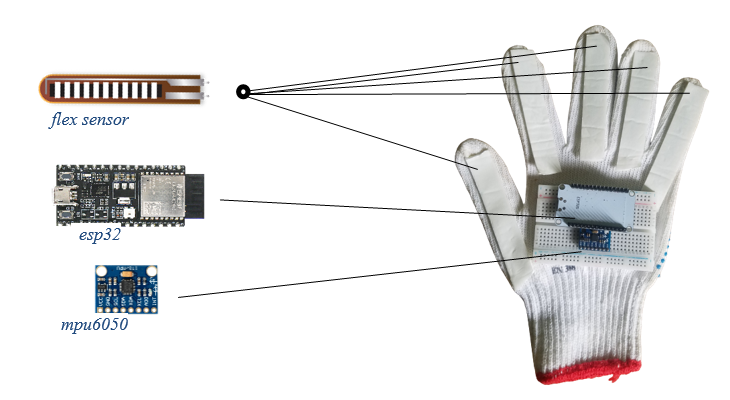
\includegraphics[width=0.8\linewidth]{images/prototype}
	\caption{TAKALEM Gloves components architecture}
	\label{fig:prototype}
\end{figure}
\subsection{ESP32 WROOM}
\paragraph{}
ESP32 is a highly versatile and powerful microcontroller \ac{soc} developed by Espressif Systems. It combines Wi-Fi and Bluetooth connectivity with a dual-core processor, making it ideal for various \ac{iot} applications.
\begin{figure}[h]
	\centering
	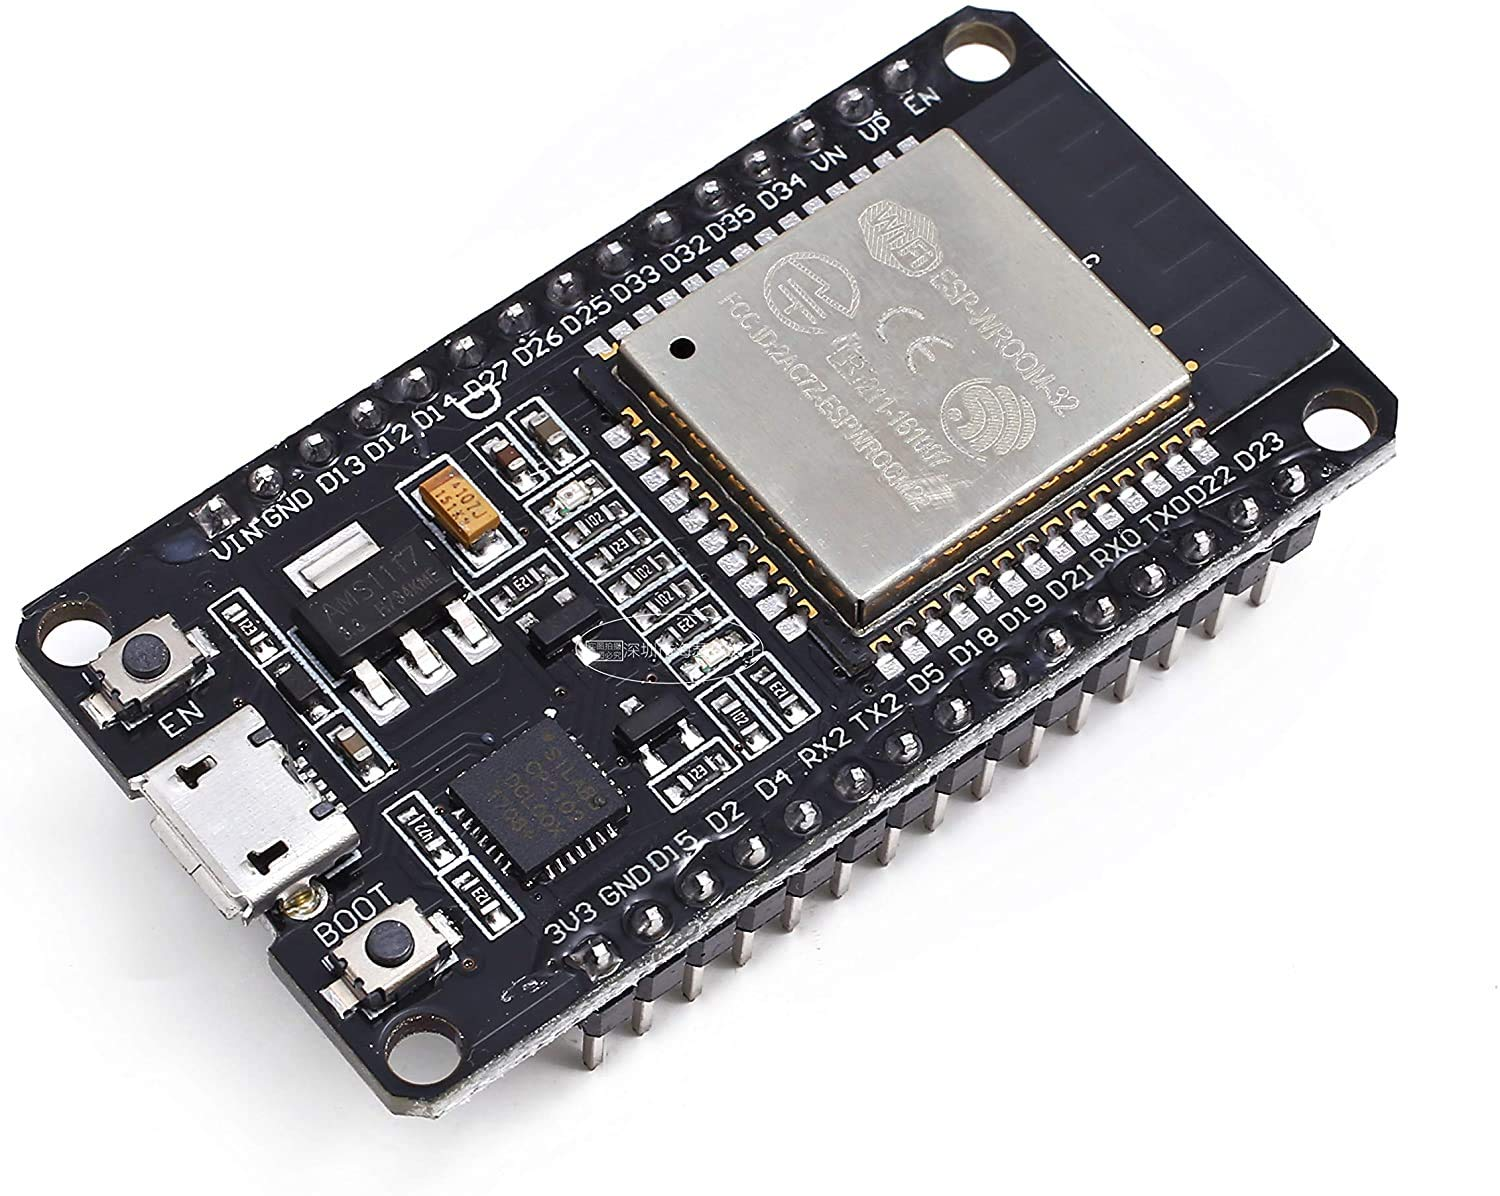
\includegraphics[width=0.6\linewidth]{images/esp32}
	\caption{ESP32 WROOM}
	\label{fig:esp32}
\end{figure}
\subsection{Flex sensor}
\paragraph{}
Flex sensor is basically a variable resistor whose terminal resistance increases when the sensor is bent. So this sensor resistance increases depends on surface linearity. So it is usually used to sense the changes in linearity "\cite{flex}.
\begin{figure}[h]
	\centering
	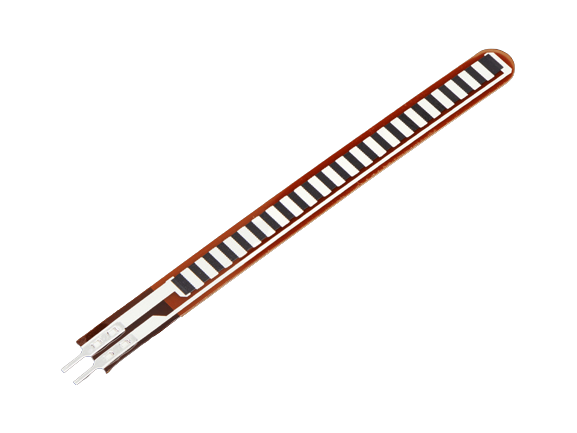
\includegraphics[width=0.6\linewidth]{images/flex-sensor}
	\caption{Flex sensor}
	\label{fig:flex-sensor}
\end{figure}
\paragraph{How flex sensor work}
As shown in figure \ref{fig:flex-cases}, when the surface of the flex sensor is completely linear it will be having its nominal resistance. When it is bent 45º angle the flex sensor resistance increases to twice as before. And when the bent is 90º the resistance could go as high as four times the nominal resistance. So the resistance across the terminals rises linearly with bent angle. So in a sense the flex sensor converts flex angle to resistance parameter "\cite{flex}.
\begin{figure}[h]
	\centering
	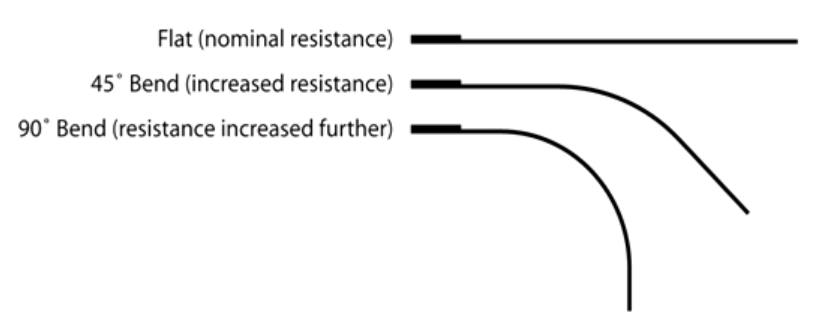
\includegraphics[width=0.6\linewidth]{images/flex-cases}
	\caption{Flex sensor cases "\cite{flex}}
	\label{fig:flex-cases}
\end{figure}
\paragraph{Flex sensor pinout}
The flex sensor is a two-way variable resistor with two pins, one for GND and the other for VCC. We wire one pin directly to the GND, the second pin is used to read the flex resistance via two wires, one is connected to the output pin in the esp32 and the other is connected to a constant resistance connected to the VCC.
\begin{figure}[h]
	\centering
	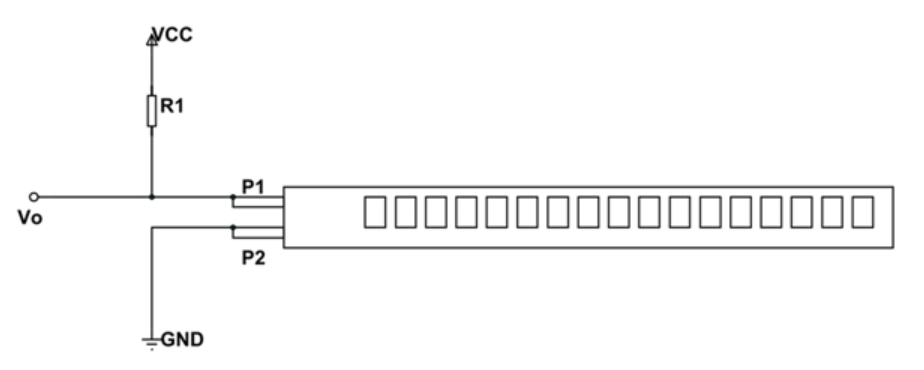
\includegraphics[width=0.6\linewidth]{images/flex-pinout}
	\caption{Flex sensor pin out}
	\label{fig:flex-pinout}
\end{figure}
\subsection{MPU6050}
\paragraph{}
The MPU6050 is a \ac{mems} which consists of a 3-axis Accelerometer and 3-axis Gyroscope inside it. This helps us to measure acceleration, velocity, orientation, displacement and many other motion related parameter of a system or object. This module also has a \ac{dmp} inside it which is powerful enough to perform complex calculation and thus free up the work for microcontrollers "\cite{mpu}.
\begin{figure}[h]
	\centering
	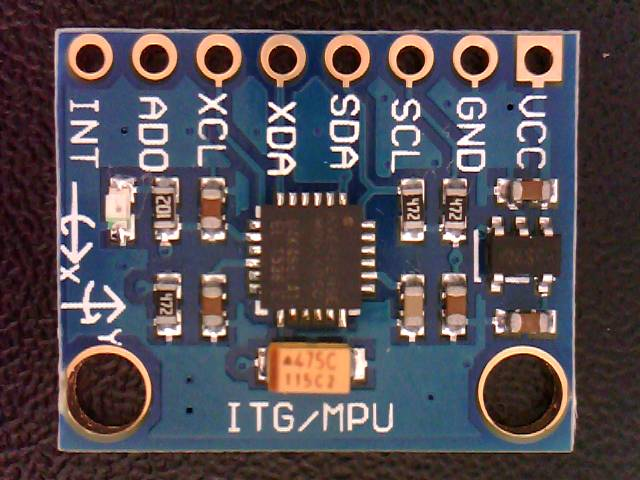
\includegraphics[width=0.6\linewidth]{images/mpu6050}
	\caption{MPU6050}
	\label{fig:mpu6050}
\end{figure}
\paragraph{MPU6050 pinout}
The MPU6050 sensor module and ESP32 have specific pinouts that need to be connected correctly. The MPU6050 typically has four important pins: VCC, GND, SDA, and SCL. The VCC pin is connected to a 3.3V or 5V output on the ESP32 to power the sensor. The GND pin of the MPU6050 is connected to a ground pin on the ESP32 to establish a common ground. The SDA pin of the MPU6050 is connected to the SDA pin on the ESP32 (pin D23), which handles the data line for I2C communication. Similarly, the SCL pin of the MPU6050 is connected to the SCL pin on the ESP32 (pin D21), which handles the clock line for I2C communication. It's important to make sure the correct pins are connected to establish proper communication between the MPU6050 and ESP32.
\begin{figure}[h]
	\centering
	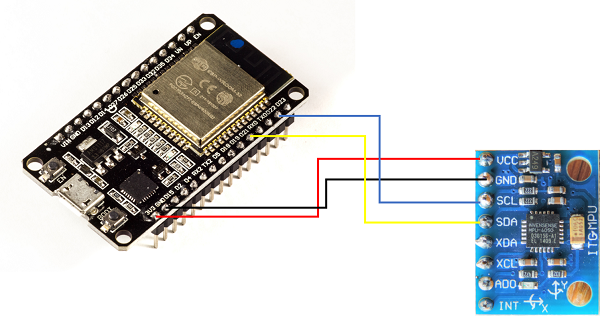
\includegraphics[width=0.6\linewidth]{images/mpu6050-pinout}
	\caption{MPU6050 pin out "\cite{mpu-pinout}}
	\label{fig:mpu6050-pinout}
\end{figure}
\section{Synthesis}
In this section, we provide a synthesis of the various methods and techniques for sign language recognition that have been discussed in section 2. We classify these methods into three categories: vision-based, sensor-based, and hybrid approaches.

Vision-based approaches rely on analyzing video data of the signer's hand gestures to recognize signs. These methods typically use computer vision techniques such as background subtraction, motion detection, and feature extraction to identify and track the signer's hands and fingers. However, vision-based approaches may face challenges such as lighting conditions, occlusion, and variability in hand shapes.

Sensor-based approaches, on the other hand, use wearable sensors to capture data on the signer's hand movements and postures. These sensors can include accelerometers, gyroscopes, flex sensors, and force sensors. Sensor-based approaches have the advantage of being more robust to lighting conditions and occlusion than vision-based approaches. However, they require careful calibration and placement of sensors on the glove or other wearable device.

Hybrid approaches combine both vision-based and sensor-based methods to improve accuracy and robustness. For example, some systems use vision-based methods to detect the signer's hand location and then switch to sensor-based methods for gesture recognition. Other systems use sensor-based methods for fine-grained gesture recognition and vision-based methods for coarse-grained gesture recognition.

Overall, there is no single best approach for sign language recognition, and the choice of method depends on the specific requirements and constraints of the application.
\section{Conclusion}
\paragraph{}
In conclusion, the analysis and synthesis of related works provide a comprehensive overview of the state of the art in \ac{slr}. The advancements in computer vision, \ac{ml}, and \ac{dl} techniques have paved the way for more accurate and efficient recognition of \ac{sl} gestures. However, there are still challenges to overcome, and further research is needed to address the limitations and improve the usability of \ac{slr} systems.
\section{Evaluation criteria}
\paragraph{}
In this section, we discuss the evaluation criteria used to assess the performance and effectiveness of the TAKALEM Gloves system for \ac{slr}. Evaluating the system's performance is crucial to understanding its strengths, limitations, and areas for improvement.
\subsection{Accuracy}
\paragraph{}
Accuracy is a fundamental metric used to evaluate the performance of sign language recognition systems. It measures the system's ability to correctly classify and interpret sign language gestures. In the context of the Takalem Gloves system, accuracy refers to the percentage of correctly recognized signs out of the total number of signs in the dataset. It can be calculated as in Eq. \ref{eq:accuracy}:
\begin{equation}
	Accuracy = \frac{TP + TN}{TP + TN + FP + FN} \label{eq:accuracy}
\end{equation}
Where:
\begin{itemize}
	\item TP represents true positive, the number of correctly recognized signs.
	\item TN represents true negative, the number of correctly rejected non-target signs.
	\item FP represents false positive, the number of incorrectly recognized signs.
	\item FN represents false negative, the number of incorrectly rejected target signs.
\end{itemize}
\subsection{Precision and macro-average precision}
\paragraph{}
Precision and recall are commonly used metrics to assess the performance of classification models. In the context of \ac{slr}, precision refers to the proportion of correctly classified signs for a specific class (e.g., individual letters or words) out of all the signs predicted as that class. Recall measures the proportion of correctly classified signs for a specific class out of all the signs that actually belong to that class. They can be calculated as in Eq. \ref{eq:precision} and Eq. \ref{eq:recall}:
\begin{equation}
	Precision = \frac{TP}{TP + FP} \label{eq:precision}
\end{equation}
\begin{equation}
	Recall = \frac{TP}{TP + FN} \label{eq:precision-macro}
\end{equation}
\subsection{Recall and macro-average recall}
\paragraph{}
Precision and recall are commonly used metrics to assess the performance of classification models. In the context of \ac{slr}, precision refers to the proportion of correctly classified signs for a specific class (e.g., individual letters or words) out of all the signs predicted as that class. Recall measures the proportion of correctly classified signs for a specific class out of all the signs that actually belong to that class. They can be calculated as in Eq. \ref{eq:precision} and Eq. \ref{eq:recall}:
\begin{equation}
	Precision = \frac{TP}{TP + FP} \label{eq:recall}
\end{equation}
\begin{equation}
	Recall = \frac{TP}{TP + FN} \label{eq:recall-macro}
\end{equation}
\subsection{F1 score and macro-average f1 score}
\paragraph{}
Precision and recall are commonly used metrics to assess the performance of classification models. In the context of \ac{slr}, precision refers to the proportion of correctly classified signs for a specific class (e.g., individual letters or words) out of all the signs predicted as that class. Recall measures the proportion of correctly classified signs for a specific class out of all the signs that actually belong to that class. They can be calculated as in Eq. \ref{eq:precision} and Eq. \ref{eq:recall}:
\begin{equation}
	Precision = \frac{TP}{TP + FP} \label{eq:f1}
\end{equation}
\begin{equation}
	Recall = \frac{TP}{TP + FN} \label{eq:f1-macro}
\end{equation}
\paragraph{}
By employing these evaluation criteria, including accuracy, precision, recall, F1 score, we can comprehensively assess the performance and capabilities of the TAKALEM Gloves system for \ac{slr}. The combination of these metrics enables us to gain a holistic understanding of the system's effectiveness, identify areas for improvement, and guide future enhancements in the field of \ac{slr} technology.

\chapter{Related works}
\section{Introduction}
In this chapter, we provide an overview of the related works in the field of sign language recognition (SLR). Sign language recognition is an important task that has gained much attention in recent years due to its potential to help improve communication between deaf and hearing individuals. The goal of SLR is to automatically recognize signs and gestures made by a person using a sign language. This is a challenging task due to the complexity and variability of sign languages, as well as the limitations of the sensing technology used to capture the movements.

The objective of this chapter is to review the state of the art in SLR, focusing on the different methods and techniques used to recognize sign language. We begin by discussing the different types of sign languages and their characteristics. We then present an overview of the different techniques used in SLR, including computer vision-based methods, data glove-based methods, and sensor-based methods. Finally, we conclude with a summary of the challenges and open problems in the field, highlighting the gaps in the existing literature and motivating the need for further research.
\section{Hardware architecture and configuration}
\paragraph{}
The TAKALEM Gloves, designed for \ac{slr}, consist of two main units: the sensing unit and the processing unit. This section focuses on the hardware architecture and configuration of these units, providing an overview of the components and their interconnections.
\paragraph{}
The sensing unit of the TAKALEM Gloves is responsible for capturing and collecting data related to hand movements and gestures. It comprises flex sensors and an MPU6050 sensor. The flex sensors are strategically positioned on the glove to measure the bend of individual fingers. They are connected to the microcontroller through designated pins, namely pins 13, 15, 25, 26, and 27. These flex sensors provide precise and real-time measurements of finger movements, allowing for accurate interpretation of \ac{sl} gestures.
\paragraph{}
In addition to the flex sensors, the TAKALEM Gloves also incorporate the MPU6050 sensor. The MPU6050 is an \ac{imu} that combines a three-axis accelerometer and a three-axis gyroscope. It measures the orientation and acceleration of the hand, providing valuable data for the \ac{slr} process. This sensor is connected to the microcontroller via the ASL (Accelerometer Serial Interface) and ASD (Accelerometer Serial Data) pins, enabling seamless data communication between the sensor and the processing unit.
\paragraph{}
The processing unit of the TAKALEM Gloves is powered by the ESP32 WROOM Module, a powerful microcontroller that integrates Wi-Fi and Bluetooth functionalities. This module acts as the brain of the gloves, processing the data collected from the flex sensors and the MPU6050 sensor. It is responsible for extracting and analyzing the sensor data, applying signal processing techniques, and calling the \ac{dl} model to predict the corresponding sign.
\paragraph{}
The ESP32 WROOM Module is equipped with sufficient computational power and memory to handle the complex algorithms and computations involved in real-time \ac{slr}. Its connectivity features allow for seamless integration with other devices, such as smartphones or smart home systems, enabling a wide range of applications.
\paragraph{}
To ensure optimal performance and reliable data transmission, the hardware components are carefully configured and calibrated. The flex sensors are positioned and secured on the glove to accurately measure finger bend without hindering natural hand movements. The MPU6050 sensor is properly calibrated to provide accurate orientation and acceleration data.
\paragraph{}
As a visual representation of the TAKALEM Gloves, \ref{fig:prototype} showcases the prototype of the gloves, highlighting the positioning of the flex sensors and the MPU6050 sensor. This prototype serves as a physical embodiment of the hardware architecture described in this section.
\begin{figure}[h]
	\centering
	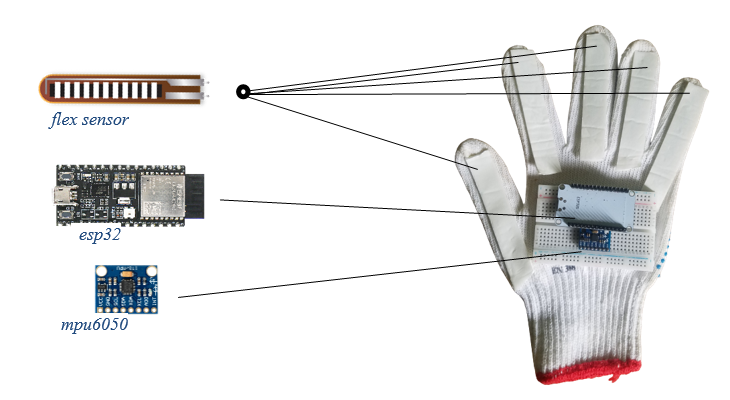
\includegraphics[width=0.8\linewidth]{images/prototype}
	\caption{TAKALEM Gloves components architecture}
	\label{fig:prototype}
\end{figure}
\subsection{ESP32 WROOM}
\paragraph{}
ESP32 is a highly versatile and powerful microcontroller \ac{soc} developed by Espressif Systems. It combines Wi-Fi and Bluetooth connectivity with a dual-core processor, making it ideal for various \ac{iot} applications.
\begin{figure}[h]
	\centering
	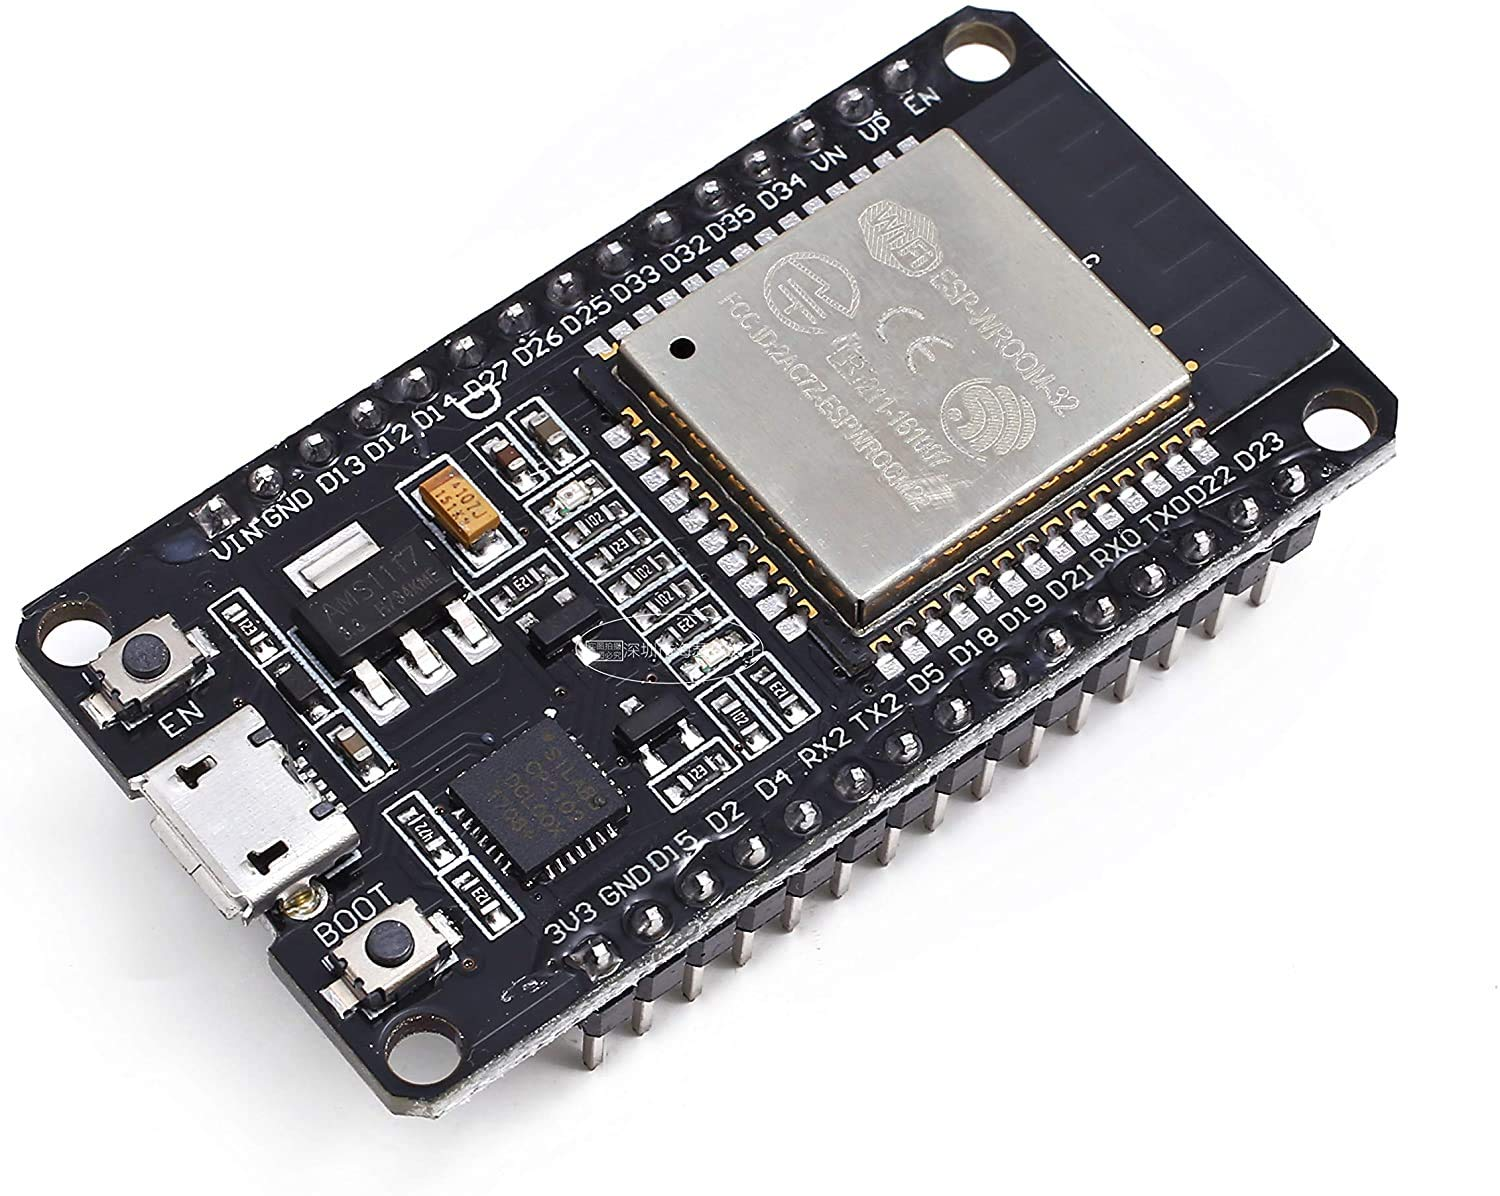
\includegraphics[width=0.6\linewidth]{images/esp32}
	\caption{ESP32 WROOM}
	\label{fig:esp32}
\end{figure}
\subsection{Flex sensor}
\paragraph{}
Flex sensor is basically a variable resistor whose terminal resistance increases when the sensor is bent. So this sensor resistance increases depends on surface linearity. So it is usually used to sense the changes in linearity "\cite{flex}.
\begin{figure}[h]
	\centering
	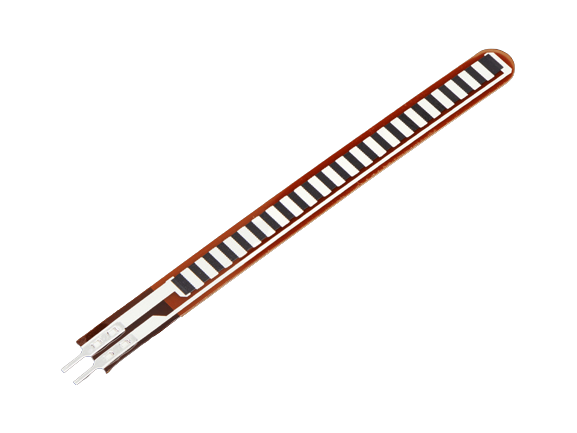
\includegraphics[width=0.6\linewidth]{images/flex-sensor}
	\caption{Flex sensor}
	\label{fig:flex-sensor}
\end{figure}
\paragraph{How flex sensor work}
As shown in figure \ref{fig:flex-cases}, when the surface of the flex sensor is completely linear it will be having its nominal resistance. When it is bent 45º angle the flex sensor resistance increases to twice as before. And when the bent is 90º the resistance could go as high as four times the nominal resistance. So the resistance across the terminals rises linearly with bent angle. So in a sense the flex sensor converts flex angle to resistance parameter "\cite{flex}.
\begin{figure}[h]
	\centering
	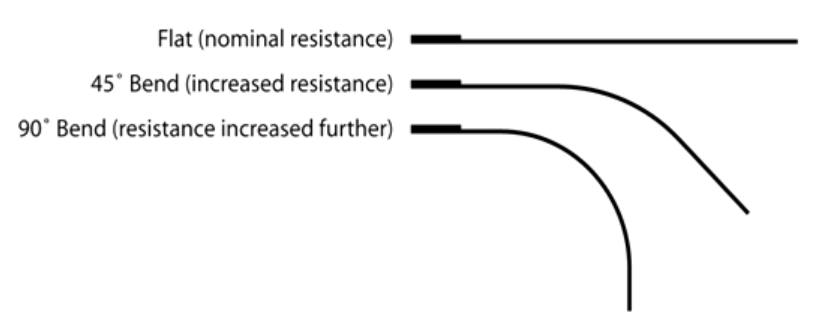
\includegraphics[width=0.6\linewidth]{images/flex-cases}
	\caption{Flex sensor cases "\cite{flex}}
	\label{fig:flex-cases}
\end{figure}
\paragraph{Flex sensor pinout}
The flex sensor is a two-way variable resistor with two pins, one for GND and the other for VCC. We wire one pin directly to the GND, the second pin is used to read the flex resistance via two wires, one is connected to the output pin in the esp32 and the other is connected to a constant resistance connected to the VCC.
\begin{figure}[h]
	\centering
	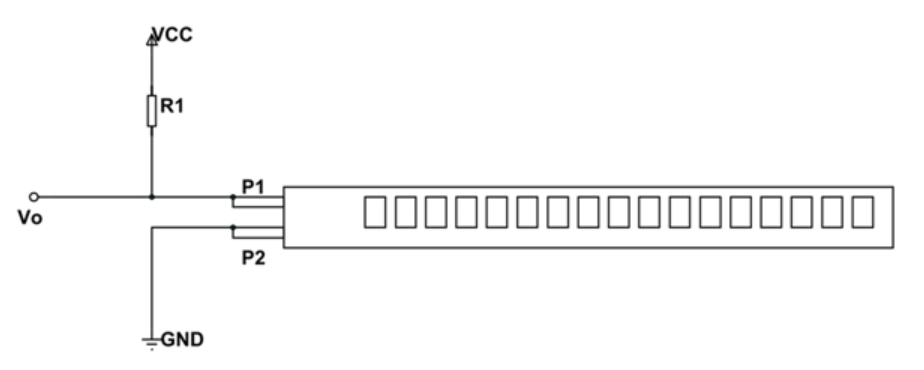
\includegraphics[width=0.6\linewidth]{images/flex-pinout}
	\caption{Flex sensor pin out}
	\label{fig:flex-pinout}
\end{figure}
\subsection{MPU6050}
\paragraph{}
The MPU6050 is a \ac{mems} which consists of a 3-axis Accelerometer and 3-axis Gyroscope inside it. This helps us to measure acceleration, velocity, orientation, displacement and many other motion related parameter of a system or object. This module also has a \ac{dmp} inside it which is powerful enough to perform complex calculation and thus free up the work for microcontrollers "\cite{mpu}.
\begin{figure}[h]
	\centering
	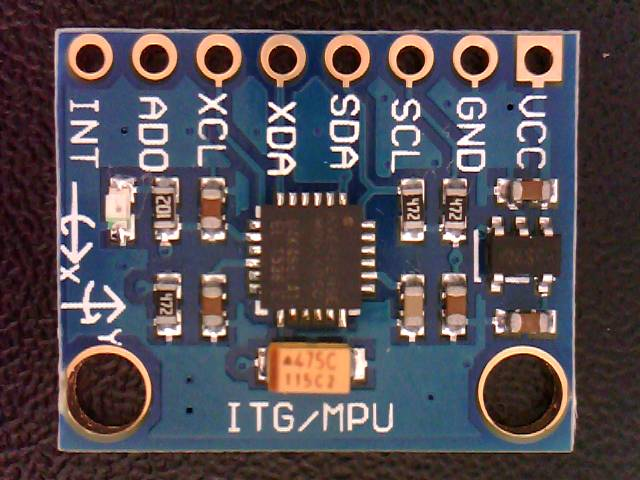
\includegraphics[width=0.6\linewidth]{images/mpu6050}
	\caption{MPU6050}
	\label{fig:mpu6050}
\end{figure}
\paragraph{MPU6050 pinout}
The MPU6050 sensor module and ESP32 have specific pinouts that need to be connected correctly. The MPU6050 typically has four important pins: VCC, GND, SDA, and SCL. The VCC pin is connected to a 3.3V or 5V output on the ESP32 to power the sensor. The GND pin of the MPU6050 is connected to a ground pin on the ESP32 to establish a common ground. The SDA pin of the MPU6050 is connected to the SDA pin on the ESP32 (pin D23), which handles the data line for I2C communication. Similarly, the SCL pin of the MPU6050 is connected to the SCL pin on the ESP32 (pin D21), which handles the clock line for I2C communication. It's important to make sure the correct pins are connected to establish proper communication between the MPU6050 and ESP32.
\begin{figure}[h]
	\centering
	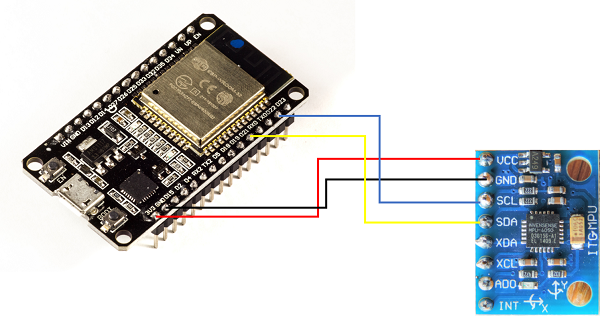
\includegraphics[width=0.6\linewidth]{images/mpu6050-pinout}
	\caption{MPU6050 pin out "\cite{mpu-pinout}}
	\label{fig:mpu6050-pinout}
\end{figure}
\section{Synthesis}
In this section, we provide a synthesis of the various methods and techniques for sign language recognition that have been discussed in section 2. We classify these methods into three categories: vision-based, sensor-based, and hybrid approaches.

Vision-based approaches rely on analyzing video data of the signer's hand gestures to recognize signs. These methods typically use computer vision techniques such as background subtraction, motion detection, and feature extraction to identify and track the signer's hands and fingers. However, vision-based approaches may face challenges such as lighting conditions, occlusion, and variability in hand shapes.

Sensor-based approaches, on the other hand, use wearable sensors to capture data on the signer's hand movements and postures. These sensors can include accelerometers, gyroscopes, flex sensors, and force sensors. Sensor-based approaches have the advantage of being more robust to lighting conditions and occlusion than vision-based approaches. However, they require careful calibration and placement of sensors on the glove or other wearable device.

Hybrid approaches combine both vision-based and sensor-based methods to improve accuracy and robustness. For example, some systems use vision-based methods to detect the signer's hand location and then switch to sensor-based methods for gesture recognition. Other systems use sensor-based methods for fine-grained gesture recognition and vision-based methods for coarse-grained gesture recognition.

Overall, there is no single best approach for sign language recognition, and the choice of method depends on the specific requirements and constraints of the application.
\section{Conclusion}
\paragraph{}
In conclusion, the analysis and synthesis of related works provide a comprehensive overview of the state of the art in \ac{slr}. The advancements in computer vision, \ac{ml}, and \ac{dl} techniques have paved the way for more accurate and efficient recognition of \ac{sl} gestures. However, there are still challenges to overcome, and further research is needed to address the limitations and improve the usability of \ac{slr} systems.

	\clearpage
	\part{Contribution}
\chapter{Conception of TAKALEM gloves}
\section{Introduction}
In this chapter, we provide an overview of the related works in the field of sign language recognition (SLR). Sign language recognition is an important task that has gained much attention in recent years due to its potential to help improve communication between deaf and hearing individuals. The goal of SLR is to automatically recognize signs and gestures made by a person using a sign language. This is a challenging task due to the complexity and variability of sign languages, as well as the limitations of the sensing technology used to capture the movements.

The objective of this chapter is to review the state of the art in SLR, focusing on the different methods and techniques used to recognize sign language. We begin by discussing the different types of sign languages and their characteristics. We then present an overview of the different techniques used in SLR, including computer vision-based methods, data glove-based methods, and sensor-based methods. Finally, we conclude with a summary of the challenges and open problems in the field, highlighting the gaps in the existing literature and motivating the need for further research.
\section{Hardware architecture and configuration}
\paragraph{}
The TAKALEM Gloves, designed for \ac{slr}, consist of two main units: the sensing unit and the processing unit. This section focuses on the hardware architecture and configuration of these units, providing an overview of the components and their interconnections.
\paragraph{}
The sensing unit of the TAKALEM Gloves is responsible for capturing and collecting data related to hand movements and gestures. It comprises flex sensors and an MPU6050 sensor. The flex sensors are strategically positioned on the glove to measure the bend of individual fingers. They are connected to the microcontroller through designated pins, namely pins 13, 15, 25, 26, and 27. These flex sensors provide precise and real-time measurements of finger movements, allowing for accurate interpretation of \ac{sl} gestures.
\paragraph{}
In addition to the flex sensors, the TAKALEM Gloves also incorporate the MPU6050 sensor. The MPU6050 is an \ac{imu} that combines a three-axis accelerometer and a three-axis gyroscope. It measures the orientation and acceleration of the hand, providing valuable data for the \ac{slr} process. This sensor is connected to the microcontroller via the ASL (Accelerometer Serial Interface) and ASD (Accelerometer Serial Data) pins, enabling seamless data communication between the sensor and the processing unit.
\paragraph{}
The processing unit of the TAKALEM Gloves is powered by the ESP32 WROOM Module, a powerful microcontroller that integrates Wi-Fi and Bluetooth functionalities. This module acts as the brain of the gloves, processing the data collected from the flex sensors and the MPU6050 sensor. It is responsible for extracting and analyzing the sensor data, applying signal processing techniques, and calling the \ac{dl} model to predict the corresponding sign.
\paragraph{}
The ESP32 WROOM Module is equipped with sufficient computational power and memory to handle the complex algorithms and computations involved in real-time \ac{slr}. Its connectivity features allow for seamless integration with other devices, such as smartphones or smart home systems, enabling a wide range of applications.
\paragraph{}
To ensure optimal performance and reliable data transmission, the hardware components are carefully configured and calibrated. The flex sensors are positioned and secured on the glove to accurately measure finger bend without hindering natural hand movements. The MPU6050 sensor is properly calibrated to provide accurate orientation and acceleration data.
\paragraph{}
As a visual representation of the TAKALEM Gloves, \ref{fig:prototype} showcases the prototype of the gloves, highlighting the positioning of the flex sensors and the MPU6050 sensor. This prototype serves as a physical embodiment of the hardware architecture described in this section.
\begin{figure}[h]
	\centering
	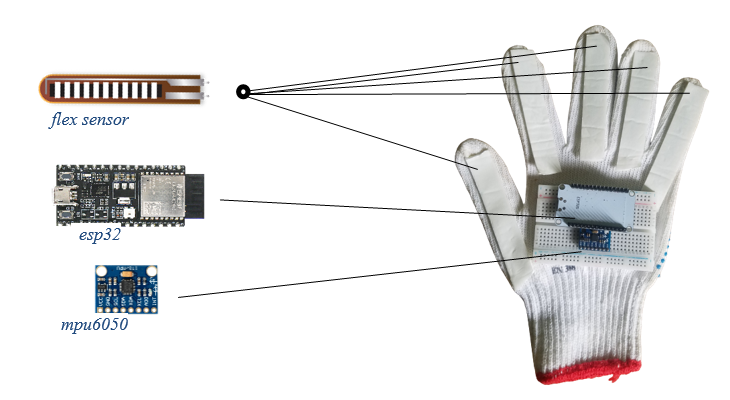
\includegraphics[width=0.8\linewidth]{images/prototype}
	\caption{TAKALEM Gloves components architecture}
	\label{fig:prototype}
\end{figure}
\subsection{ESP32 WROOM}
\paragraph{}
ESP32 is a highly versatile and powerful microcontroller \ac{soc} developed by Espressif Systems. It combines Wi-Fi and Bluetooth connectivity with a dual-core processor, making it ideal for various \ac{iot} applications.
\begin{figure}[h]
	\centering
	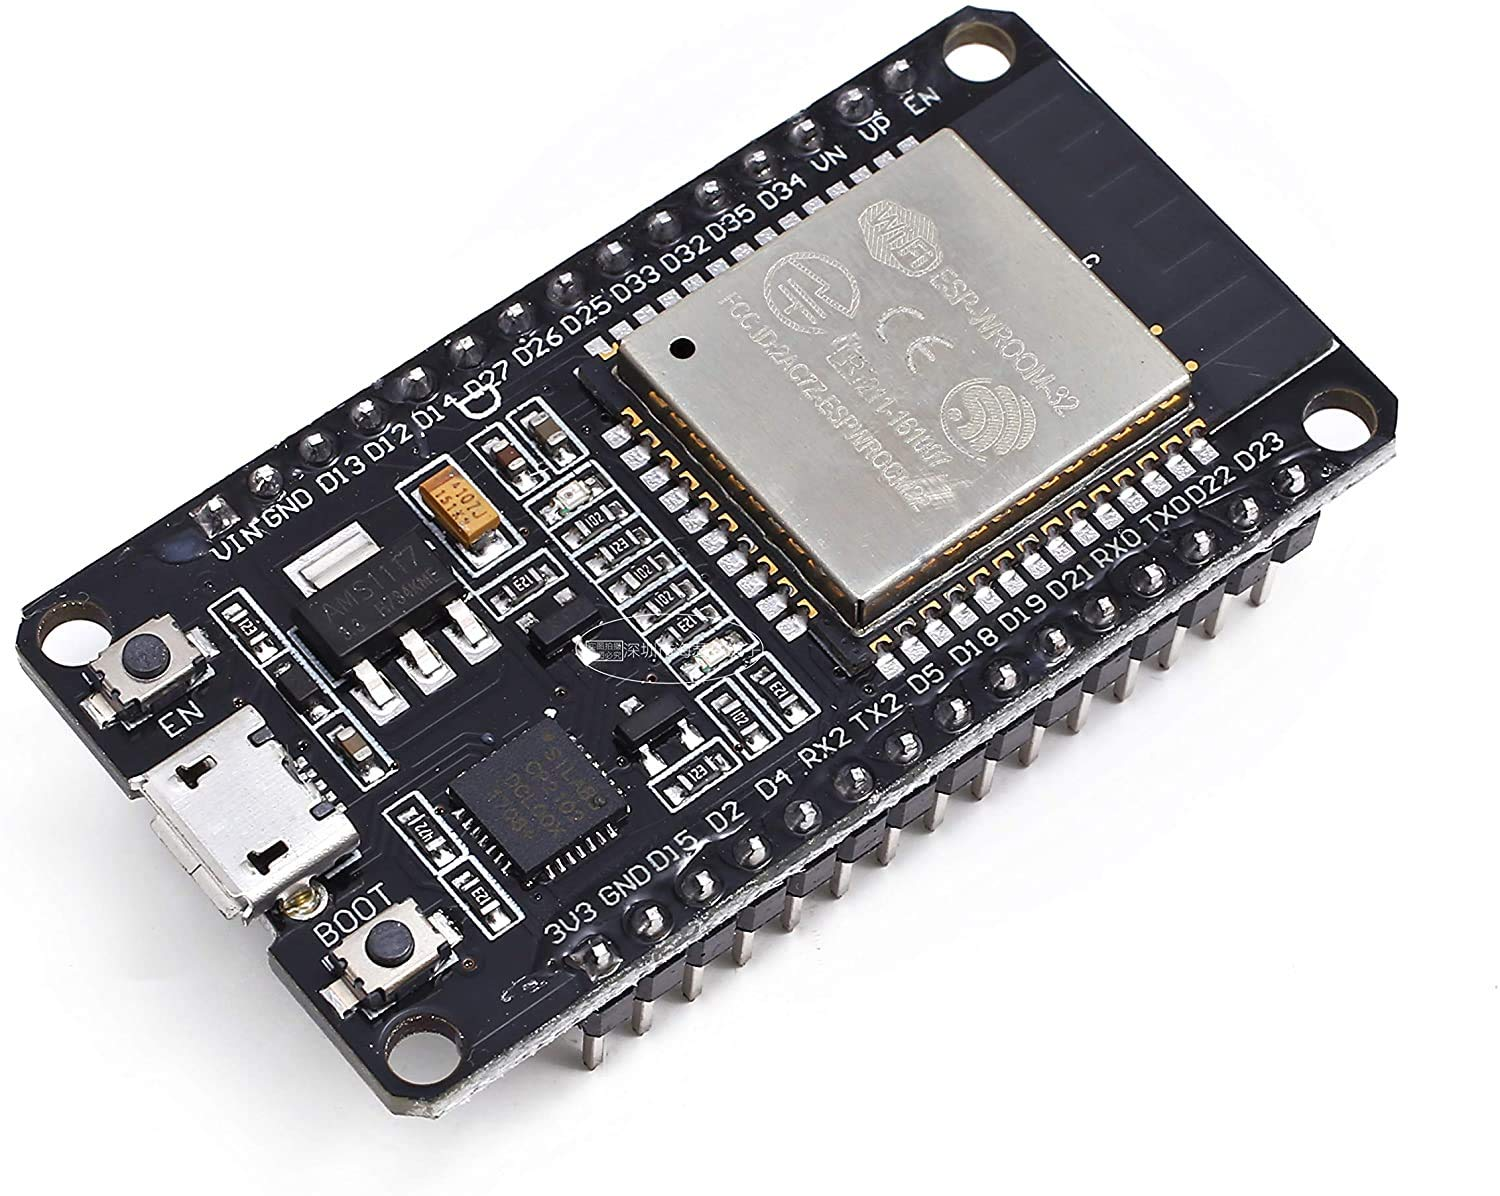
\includegraphics[width=0.6\linewidth]{images/esp32}
	\caption{ESP32 WROOM}
	\label{fig:esp32}
\end{figure}
\subsection{Flex sensor}
\paragraph{}
Flex sensor is basically a variable resistor whose terminal resistance increases when the sensor is bent. So this sensor resistance increases depends on surface linearity. So it is usually used to sense the changes in linearity "\cite{flex}.
\begin{figure}[h]
	\centering
	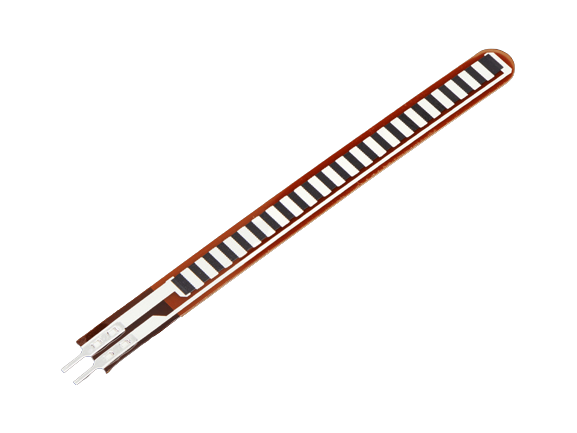
\includegraphics[width=0.6\linewidth]{images/flex-sensor}
	\caption{Flex sensor}
	\label{fig:flex-sensor}
\end{figure}
\paragraph{How flex sensor work}
As shown in figure \ref{fig:flex-cases}, when the surface of the flex sensor is completely linear it will be having its nominal resistance. When it is bent 45º angle the flex sensor resistance increases to twice as before. And when the bent is 90º the resistance could go as high as four times the nominal resistance. So the resistance across the terminals rises linearly with bent angle. So in a sense the flex sensor converts flex angle to resistance parameter "\cite{flex}.
\begin{figure}[h]
	\centering
	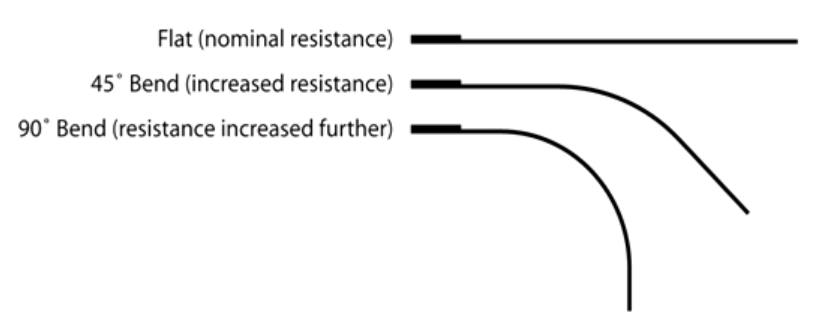
\includegraphics[width=0.6\linewidth]{images/flex-cases}
	\caption{Flex sensor cases "\cite{flex}}
	\label{fig:flex-cases}
\end{figure}
\paragraph{Flex sensor pinout}
The flex sensor is a two-way variable resistor with two pins, one for GND and the other for VCC. We wire one pin directly to the GND, the second pin is used to read the flex resistance via two wires, one is connected to the output pin in the esp32 and the other is connected to a constant resistance connected to the VCC.
\begin{figure}[h]
	\centering
	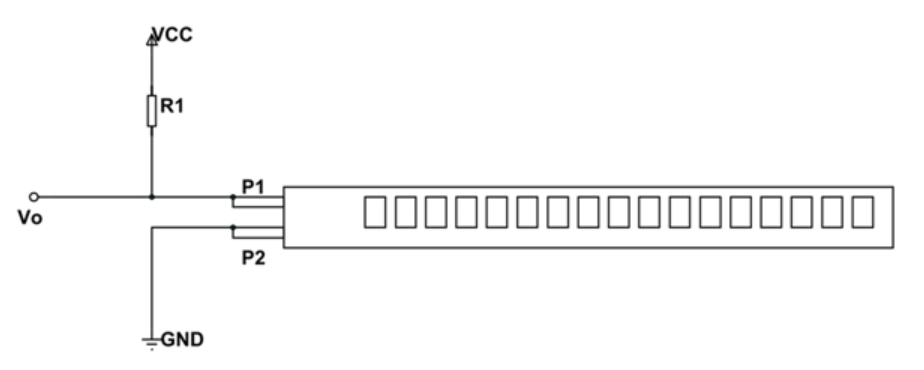
\includegraphics[width=0.6\linewidth]{images/flex-pinout}
	\caption{Flex sensor pin out}
	\label{fig:flex-pinout}
\end{figure}
\subsection{MPU6050}
\paragraph{}
The MPU6050 is a \ac{mems} which consists of a 3-axis Accelerometer and 3-axis Gyroscope inside it. This helps us to measure acceleration, velocity, orientation, displacement and many other motion related parameter of a system or object. This module also has a \ac{dmp} inside it which is powerful enough to perform complex calculation and thus free up the work for microcontrollers "\cite{mpu}.
\begin{figure}[h]
	\centering
	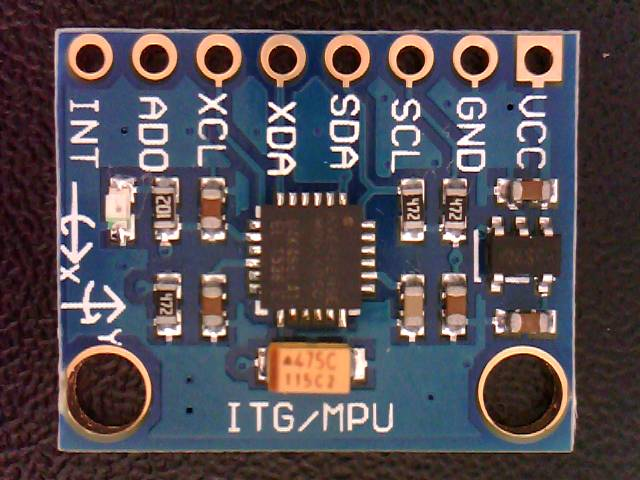
\includegraphics[width=0.6\linewidth]{images/mpu6050}
	\caption{MPU6050}
	\label{fig:mpu6050}
\end{figure}
\paragraph{MPU6050 pinout}
The MPU6050 sensor module and ESP32 have specific pinouts that need to be connected correctly. The MPU6050 typically has four important pins: VCC, GND, SDA, and SCL. The VCC pin is connected to a 3.3V or 5V output on the ESP32 to power the sensor. The GND pin of the MPU6050 is connected to a ground pin on the ESP32 to establish a common ground. The SDA pin of the MPU6050 is connected to the SDA pin on the ESP32 (pin D23), which handles the data line for I2C communication. Similarly, the SCL pin of the MPU6050 is connected to the SCL pin on the ESP32 (pin D21), which handles the clock line for I2C communication. It's important to make sure the correct pins are connected to establish proper communication between the MPU6050 and ESP32.
\begin{figure}[h]
	\centering
	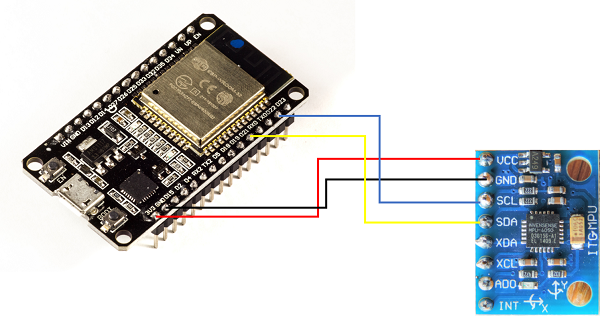
\includegraphics[width=0.6\linewidth]{images/mpu6050-pinout}
	\caption{MPU6050 pin out "\cite{mpu-pinout}}
	\label{fig:mpu6050-pinout}
\end{figure}
\section{Synthesis}
In this section, we provide a synthesis of the various methods and techniques for sign language recognition that have been discussed in section 2. We classify these methods into three categories: vision-based, sensor-based, and hybrid approaches.

Vision-based approaches rely on analyzing video data of the signer's hand gestures to recognize signs. These methods typically use computer vision techniques such as background subtraction, motion detection, and feature extraction to identify and track the signer's hands and fingers. However, vision-based approaches may face challenges such as lighting conditions, occlusion, and variability in hand shapes.

Sensor-based approaches, on the other hand, use wearable sensors to capture data on the signer's hand movements and postures. These sensors can include accelerometers, gyroscopes, flex sensors, and force sensors. Sensor-based approaches have the advantage of being more robust to lighting conditions and occlusion than vision-based approaches. However, they require careful calibration and placement of sensors on the glove or other wearable device.

Hybrid approaches combine both vision-based and sensor-based methods to improve accuracy and robustness. For example, some systems use vision-based methods to detect the signer's hand location and then switch to sensor-based methods for gesture recognition. Other systems use sensor-based methods for fine-grained gesture recognition and vision-based methods for coarse-grained gesture recognition.

Overall, there is no single best approach for sign language recognition, and the choice of method depends on the specific requirements and constraints of the application.
\section{Conclusion}
\paragraph{}
In conclusion, the analysis and synthesis of related works provide a comprehensive overview of the state of the art in \ac{slr}. The advancements in computer vision, \ac{ml}, and \ac{dl} techniques have paved the way for more accurate and efficient recognition of \ac{sl} gestures. However, there are still challenges to overcome, and further research is needed to address the limitations and improve the usability of \ac{slr} systems.
\section{Evaluation criteria}
\paragraph{}
In this section, we discuss the evaluation criteria used to assess the performance and effectiveness of the TAKALEM Gloves system for \ac{slr}. Evaluating the system's performance is crucial to understanding its strengths, limitations, and areas for improvement.
\subsection{Accuracy}
\paragraph{}
Accuracy is a fundamental metric used to evaluate the performance of sign language recognition systems. It measures the system's ability to correctly classify and interpret sign language gestures. In the context of the Takalem Gloves system, accuracy refers to the percentage of correctly recognized signs out of the total number of signs in the dataset. It can be calculated as in Eq. \ref{eq:accuracy}:
\begin{equation}
	Accuracy = \frac{TP + TN}{TP + TN + FP + FN} \label{eq:accuracy}
\end{equation}
Where:
\begin{itemize}
	\item TP represents true positive, the number of correctly recognized signs.
	\item TN represents true negative, the number of correctly rejected non-target signs.
	\item FP represents false positive, the number of incorrectly recognized signs.
	\item FN represents false negative, the number of incorrectly rejected target signs.
\end{itemize}
\subsection{Precision and macro-average precision}
\paragraph{}
Precision and recall are commonly used metrics to assess the performance of classification models. In the context of \ac{slr}, precision refers to the proportion of correctly classified signs for a specific class (e.g., individual letters or words) out of all the signs predicted as that class. Recall measures the proportion of correctly classified signs for a specific class out of all the signs that actually belong to that class. They can be calculated as in Eq. \ref{eq:precision} and Eq. \ref{eq:recall}:
\begin{equation}
	Precision = \frac{TP}{TP + FP} \label{eq:precision}
\end{equation}
\begin{equation}
	Recall = \frac{TP}{TP + FN} \label{eq:precision-macro}
\end{equation}
\subsection{Recall and macro-average recall}
\paragraph{}
Precision and recall are commonly used metrics to assess the performance of classification models. In the context of \ac{slr}, precision refers to the proportion of correctly classified signs for a specific class (e.g., individual letters or words) out of all the signs predicted as that class. Recall measures the proportion of correctly classified signs for a specific class out of all the signs that actually belong to that class. They can be calculated as in Eq. \ref{eq:precision} and Eq. \ref{eq:recall}:
\begin{equation}
	Precision = \frac{TP}{TP + FP} \label{eq:recall}
\end{equation}
\begin{equation}
	Recall = \frac{TP}{TP + FN} \label{eq:recall-macro}
\end{equation}
\subsection{F1 score and macro-average f1 score}
\paragraph{}
Precision and recall are commonly used metrics to assess the performance of classification models. In the context of \ac{slr}, precision refers to the proportion of correctly classified signs for a specific class (e.g., individual letters or words) out of all the signs predicted as that class. Recall measures the proportion of correctly classified signs for a specific class out of all the signs that actually belong to that class. They can be calculated as in Eq. \ref{eq:precision} and Eq. \ref{eq:recall}:
\begin{equation}
	Precision = \frac{TP}{TP + FP} \label{eq:f1}
\end{equation}
\begin{equation}
	Recall = \frac{TP}{TP + FN} \label{eq:f1-macro}
\end{equation}
\paragraph{}
By employing these evaluation criteria, including accuracy, precision, recall, F1 score, we can comprehensively assess the performance and capabilities of the TAKALEM Gloves system for \ac{slr}. The combination of these metrics enables us to gain a holistic understanding of the system's effectiveness, identify areas for improvement, and guide future enhancements in the field of \ac{slr} technology.
\section{Results}
\paragraph{}
In this section, we present the evaluation results for the word and character recognition models. The purpose is to assess the performance of each model and gain insights into their effectiveness.
\subsection{Word Recognition Results}
\paragraph{}
The word recognition model was evaluated using a comprehensive set of word samples. The model achieved an accuracy of 94.63\% on the test dataset. The confusion matrix, depicted in Figure \ref{fig:words_confusion_matrix}, shows the distribution of predicted labels versus the true labels for each word class.
\paragraph{}
From the confusion matrix, we can observe that the model performs remarkably well, with most of the samples being correctly classified. There are only slight errors in some cases. However, overall, the model demonstrates high accuracy and precision.
\paragraph{}
To gain a comprehensive understanding of the word recognition model's performance, we present the classification report in Figure \ref{fig:words_classification_report}.
\paragraph{}
The classification report provides insights into the precision, recall, and F1 score for each word class. The macro average precision, recall, and F1 score for the word recognition model are 94\%, 95\%, and 95\%, respectively. These results indicate the model's strong performance in correctly recognizing the majority of the word classes.
 \ref{tab:words_classification_report}.
\subsection{Character Recognition Results}
\paragraph{}
Moving on to character recognition, the model achieved an accuracy of 95.03\% on the test dataset. The confusion matrix, shown in Figure \ref{fig:characters_confusion_matrix}, illustrates the predicted labels versus the true labels for each character class.
\paragraph{}
Similar to the word recognition model, the confusion matrix for the character recognition model demonstrates excellent performance, with minimal errors. The model accurately recognizes the majority of the characters, with only slight confusion between similar characters like "u" and "v".
\paragraph{}
To gain a comprehensive understanding of the character recognition model's performance, we present the classification report in Figure \ref{tab:characters_classification_report}.
\paragraph{}
The classification report presents the precision, recall, and F1 score for each character class. The average precision, recall, and F1 score for the character recognition model are 95\% for all of them. These results indicate the model's high accuracy in correctly identifying the majority of the character classes.
\paragraph{}
In summary, both the word and character recognition models demonstrate excellent performance with an accuracy of 94.63\% and 95.03\% respectively. The confusion matrices reveal minimal errors, while the classification reports confirm the models' precision, recall, and F1 score across various word and character classes. These results indicate the effectiveness and reliability of the implemented models in \ac{slr}.
\begin{figure}[h]
	\centering
	\begin{subfigure}[b]{0.6\textwidth}
		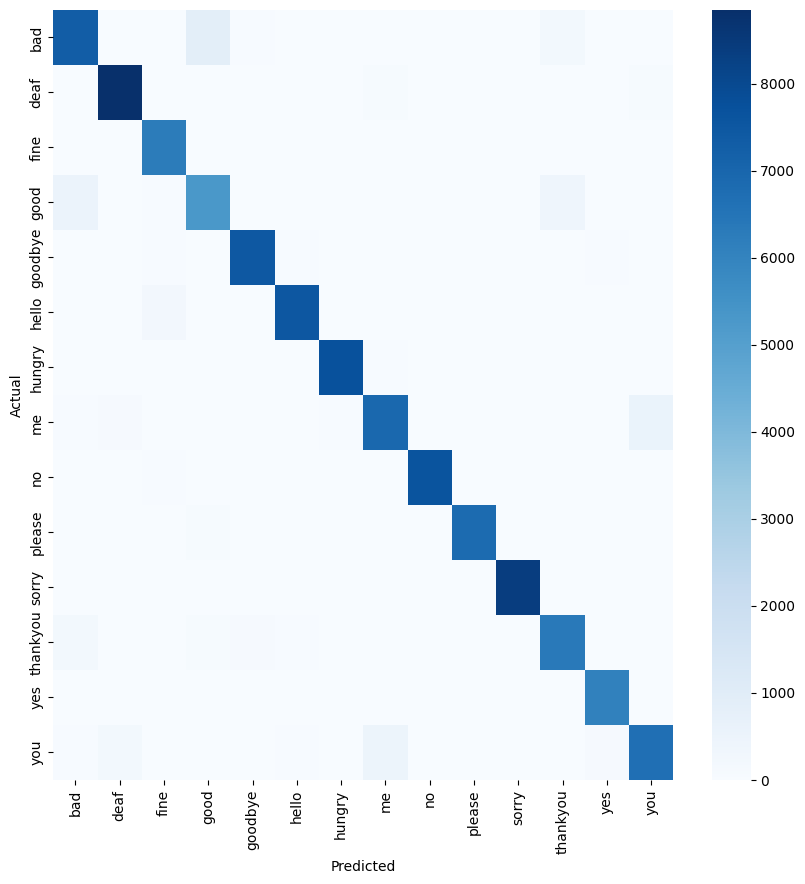
\includegraphics[width=\textwidth]{images/confusion_matrix_words}
		\caption{Confusion matrix for the word recognition model.}
		\label{fig:words_confusion_matrix}
	\end{subfigure}
	\begin{subfigure}[b]{0.6\textwidth}
		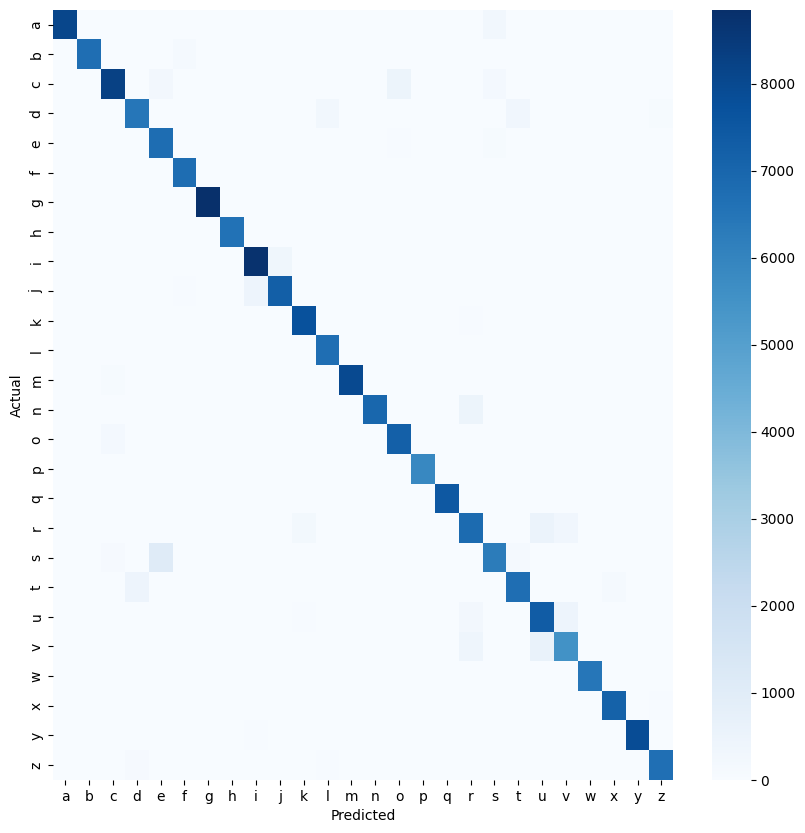
\includegraphics[width=\textwidth]{images/confusion_matrix_characters}
		\caption{Confusion matrix for character recognition model}
		\label{fig:characters_confusion_matrix}
	\end{subfigure}
	\caption{Confusion matrices}
	\label{fig:confusion_matrices}
\end{figure}
\begin{table}[h]
	\centering
	\begin{tabular}{|c|c|c|c|c|}
		\hline
		& precision & recall & f1-score & support \\
		\hline
		0 & 0.89 & 0.86 & 0.87 & 8550 \\
		\hline
		1 & 0.96 & 0.98 & 0.97 & 9000 \\
		\hline
		2 & 0.93 & 0.99 & 0.96 & 6300 \\
		\hline
		3 & 0.82 & 0.84 & 0.83 & 6300 \\
		\hline
		4 & 0.98 & 0.98 & 0.98 & 7650 \\
		\hline
		5 & 0.98 & 0.96 & 0.97 & 7800 \\
		\hline
		6 & 0.99 & 0.99 & 0.99 & 7800 \\
		\hline
		7 & 0.91 & 0.89 & 0.90 & 7800 \\
		\hline
		8 & 1.00 & 0.99 & 1.00 & 7650 \\
		\hline
		9 & 0.99 & 0.97 & 0.98 & 7050 \\
		\hline
		10 & 0.99 & 1.00 & 1.00 & 8400 \\
		\hline
		11 & 0.90 & 0.93 & 0.91 & 6900 \\
		\hline
		12 & 0.97 & 0.99 & 0.98 & 6150 \\
		\hline
		13 & 0.91 & 0.87 & 0.89 & 7650 \\
		\hline
		accuracy & - & - & 0.95 & 105000 \\
		\hline
		macro avg & 0.94 & 0.95 & 0.95 & 105000 \\
		\hline
	\end{tabular}
	\caption{Words classification report}
	\label{tab:words_classification_report}
\end{table}
\begin{table}[h]
	\centering
	\begin{tabular}{|c|c|c|c|c|}
		\hline
		& precision & recall & f1-score & support \\
		\hline
		0 & 1.00 & 0.96 & 0.98 & 8400 \\
		\hline
		1 & 1.00 & 0.98 & 0.99 & 6900 \\
		\hline
		2 & 0.95 & 0.89 & 0.92 & 9300 \\
		\hline
		3 & 0.91 & 0.89 & 0.90 & 7200 \\
		\hline
		4 & 0.83 & 0.98 & 0.90 & 6900 \\
		\hline
		5 & 0.97 & 1.00 & 0.99 & 6750 \\
		\hline
		6 & 1.00 & 1.00 & 1.00 & 8850 \\
		\hline
		7 & 1.000 & 1.00 & 1.00 & 6600 \\
		\hline
		8 & 0.94 & 0.96 & 0.95 & 9150 \\
		\hline
		9 & 0.95 & 0.93 & 0.94 & 7800 \\
		\hline
		10 & 0.96 & 0.99 & 0.97 & 7800 \\
		\hline
		11 & 0.95 & 1.00 & 0.97 & 6750 \\
		\hline
		12 & 1.00 & 0.99 & 0.99 & 8100 \\
		\hline
		13 & 0.99 & 0.93 & 0.96 & 7500 \\
		\hline
		14 & 0.93 & 0.96 & 0.94 & 7500 \\
		\hline
		15 & 1.00 & 1.00 & 1.00 & 5850 \\
		\hline
		16 & 1.00 & 1.00 & 1.00 & 7500 \\
		\hline
		17 & 0.85 & 0.86 & 0.85 & 7950 \\
		\hline
		18 & 0.91 & 0.82 & 0.86 & 7650 \\
		\hline
		19 & 0.93 & 0.91 & 0.92 & 7350 \\
		\hline
		20 & 0.86 & 0.91 & 0.88 & 8100 \\
		\hline
		21 & 0.87 & 0.83 & 0.85 & 6600 \\
		\hline
		22 & 1.00 & 1.00 & 1.00 & 6450 \\
		\hline
		23 & 0.97 & 0.99 & 0.98 & 7200 \\
		\hline
		24 & 0.99 & 0.99 & 0.99 & 7950 \\
		\hline
		25 & 0.98 & 0.97 & 0.97 & 6900 \\
		\hline
		accuracy & - & - & 0.95 & 195000 \\
		\hline
		macro avg & 0.95 & 0.95 & 0.95 & 195000 \\
		\hline
	\end{tabular}
	\caption{Characters classification report}
	\label{tab:characters_classification_report}
\end{table}
\section{Conclusion}
\paragraph{}
Our study aimed to develop a \ac{slr} model using a pre-existing sensor-based \ac{asl} dataset. Despite the time constraints and limited resources, we leveraged the \ac{asl} dataset, which consists of 40 different signs, including 26 letters and 14 common words. The dataset was collected from 25 subjects, with each subject repeating each gesture 10 times, resulting in a total of 150,000 records.
\paragraph{}
Throughout our research, we successfully trained and evaluated a \ac{dl} model for \ac{slr}. The word recognition model achieved an impressive accuracy of 94.63\% on the test dataset, while the character recognition model achieved an accuracy of 95.03\%. These results demonstrate the effectiveness and reliability of our implemented models in accurately recognizing and classifying \ac{sl} gestures.
\paragraph{}
However, it is important to acknowledge the limitations of our study. The use of an \ac{asl} dataset, instead of a dedicated \ac{asp} dataset, poses a significant limitation. While the \ac{asl} dataset provided a solid foundation for our research, it may not fully capture the unique characteristics and nuances of \ac{asp}. Future work should prioritize the collection of a dedicated dataset specific to \ac{asp} to train the model more effectively.
\paragraph{}
Furthermore, considering the limited number of subjects and gestures in our dataset, expanding the dataset with more diverse subjects and a broader range of signs would contribute to a more comprehensive and generalized \ac{slr} model.
\paragraph{}
In conclusion, our study demonstrates the potential of \ac{dl} models in \ac{slr}. Despite the limitations, our models achieved high accuracy in recognizing both words and characters from the \ac{asl} dataset. By addressing the identified limitations and incorporating additional data sources, such as dedicated \ac{asp} datasets and multiple modalities, future research can further improve the accuracy and applicability of \ac{slr} systems.

	\clearpage
	\addcontentsline{toc}{chapter}{General Conclusion}
	\chapter*{General Conclusion}
\paragraph{}
	\clearpage
	\bibliographystyle{ieeetr}
	\bibliography{includes/references}
\end{document}
